\subsection{The cone of an injective morphism; new definition of the connecting homomorphism}

Consider now an exact sequence of complexes

\[
0 \rightarrow \mathrm{C} ^ {\prime} \xrightarrow {u} \mathrm{C} \xrightarrow {v} \mathrm{C} ^ {\prime \prime} \rightarrow 0.\tag{9}
\]

Define a graded A-linear map of degree 0

\[
\varphi : \operatorname{Con} (u) \rightarrow \mathrm{C} ^ {\prime \prime}
\]

by \(\varphi(y', x) = v(x)\) . We then have a commutative diagram of A-modules with exact rows

\[
\begin{array}{c} 0 \longrightarrow \mathrm{C} ^ {\prime} \stackrel {{\tilde {u}}} {{\longrightarrow}} \mathrm{Cyl} (u) \stackrel {{\tilde {\pi}}} {{\longrightarrow}} \mathrm{Con} (u) \longrightarrow 0 \\ 1 \Big \downarrow \qquad \qquad \qquad \beta \Big \downarrow \qquad \qquad \qquad \varphi \Big \downarrow \\ 0. \longrightarrow \mathrm{C} ^ {\prime} \stackrel {{u}} {{\longrightarrow}} \mathrm{C} \stackrel {{v}} {{\longrightarrow}} \mathrm{C} ^ {\prime \prime} \longrightarrow 0. \end{array}\tag{10}
\]

PROPOSITION 9. --- The maps β and φ are homologisms of complexes. For β, this follows from prop. 7, c). We have

\[
\begin{array}{r l} \varphi \circ \mathrm{D} (y ^ {\prime}, x) & = \varphi (- d ^ {\prime} y ^ {\prime}, d x - u (y ^ {\prime})) = v (d x - u (y ^ {\prime})) \\ & = v (d x) = d ^ {\prime \prime} v (x) = d ^ {\prime \prime} (\varphi (y ^ {\prime}, x)), \end{array}
\]

hence \(\varphi\) is indeed a morphism of complexes. On the other hand, \(\varphi\) is surjective and its kernel is identified with the complex \((\mathbf{K}, d_{\mathbf{K}})\) such that \(\mathbf{K} = \mathbf{C}'(-1) \oplus \mathbf{C}'\) ,

\[
d _ {\mathbf {K}} (y ^ {\prime}, x ^ {\prime}) = (- d ^ {\prime} y ^ {\prime}, d ^ {\prime} x ^ {\prime} - y ^ {\prime});
\]

if \(d_{\mathbf{K}}(y', x') = 0\) , we have \(y' = d'x'\) , hence \((y', x') = d_{\mathbf{K}}(0, -x')\) ; it follows that \(\mathrm{H}(\mathbf{K}) = 0\) and \(\varphi\) is a homologism by X, p.~30, cor. 1.

Remark. --- The homologism β is a homotopism, but φ is not in general a homotopism (cf.~X, p.~173, exercise 8).

COROLLARY. --- The diagram of graded A-modules

\pandocbounded{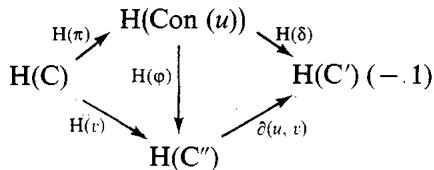
\includegraphics[keepaspectratio]{images/part001_82ee8f27.jpg}}

is commutative and H(φ) is bijective.

In the commutative diagram (10), we have \(\mathrm{H}(1_{\mathbf{C}^{\prime}})\circ \partial (\tilde{u},\tilde{\pi}) = \partial (u,v)\circ \mathrm{H}(\varphi)\) (X, p.~31, prop. 2) and \(\partial (\tilde{u},\tilde{\pi}) = \mathrm{H}(\delta)\) (X, p.~38, lemma 3, b)), hence

\[
\partial (u, v) \circ \mathbf {H} (\varphi) = \mathbf {H} (\delta);
\]

on the other hand, \(\mathrm{H}(v) \circ \mathrm{H}(\beta) = \mathrm{H}(\varphi) \circ \mathrm{H}(\tilde{\pi}) = \mathrm{H}(\varphi) \circ \mathrm{H}(\pi) \circ \mathrm{H}(\beta)\) by X, p.~39, remark. Since \(\mathrm{H}(\beta)\) is bijective, this gives \(\mathrm{H}(v) = \mathrm{H}(\varphi) \circ \mathrm{H}(\pi)\) .

We therefore have \(\partial(u, v) = H(\delta) \circ H(\varphi)^{-1}\) , which provides a new definition of the connecting homomorphism \(\partial(u, v)\) . We also note that if we identify \(H(Con(u))\) with \(H(C'')\) by \(H(\varphi)\) , the preceding corollary means that the exact sequence (8) is then identified with the exact homology sequence relative to (9).

